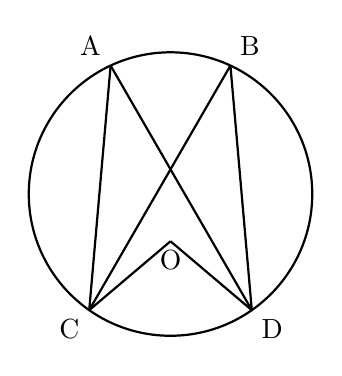
\begin{tikzpicture}[scale=1]

    % Define the radius of the circle
    \def\R{1.8}

    % Define the actual geometric center of the circle
    \coordinate (Center) at (0,0);

    % Define points A, B, C, D on the circle using polar coordinates
    \coordinate (A) at (115:\R);
    \coordinate (B) at (65:\R);
    \coordinate (C) at (235:\R);
    \coordinate (D) at (305:\R);

    % Define the point O, dragged physically further down as requested
    \coordinate (O) at (0, -0.6);

    % Draw the main circle
    \draw[thick] (Center) circle (\R);

    % Draw the line segments connecting the points on the circle to form the intersecting triangles
    \draw[thick] (A) -- (C);
    \draw[thick] (A) -- (D);
    \draw[thick] (B) -- (C);
    \draw[thick] (B) -- (D);

    % Draw the line segments from the newly dragged point O to the bottom points C and D
    \draw[thick] (O) -- (C);
    \draw[thick] (O) -- (D);

    % Add text labels to the points exactly where they appear in the image
    \node[above left] at (A) {A};
    \node[above right] at (B) {B};
    \node[below left] at (C) {C};
    \node[below right] at (D) {D};
    
    % Place the label 'O' neatly below the newly dragged coordinate
    \node[below] at (O) {O};

\end{tikzpicture}